\documentclass[11pt, oneside]{article}   	% use "amsart" instead of "article" for AMSLaTeX format
\usepackage{geometry}                		% See geometry.pdf to learn the layout options. There are lots.
\geometry{letterpaper}                   		% ... or a4paper or a5paper or ... 
%\geometry{landscape}                		% Activate for for rotated page geometry
%\usepackage[parfill]{parskip}    		% Activate to begin paragraphs with an empty line rather than an indent
\usepackage{graphicx}				% Use pdf, png, jpg, or eps� with pdflatex; use eps in DVI mode
								% TeX will automatically convert eps --> pdf in pdflatex		
\usepackage{amssymb}
\usepackage{amsmath}

\title{Parametrizing the sphere}
%\author{The Author}
%\section{}
% \subsection*{R code}
\date{}							% Activate to display a given date or no date

\graphicspath{{/Users/telliott_admin/Dropbox/Tex/png/}}

% \begin{center} 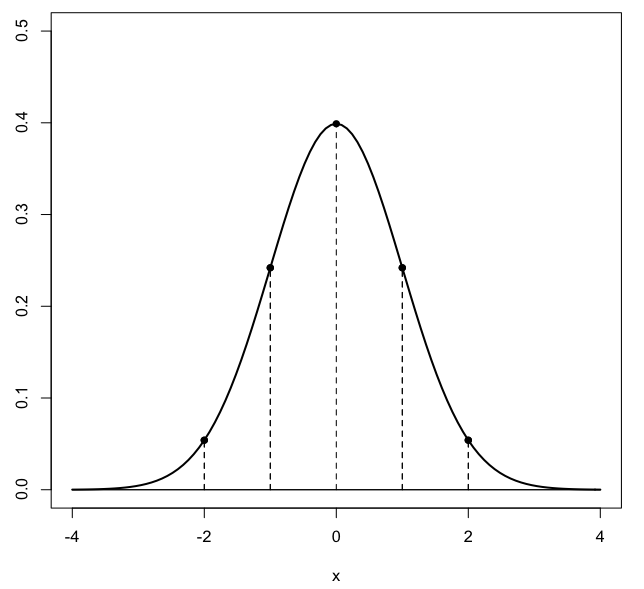
\includegraphics [scale=0.4] {gauss3.png} \end{center}
% \begin{bmatrix} a  &  b \\ c  &  d \end{bmatrix}
% \bigg |_

\begin{document}
\maketitle
\large
%\noindent
A sphere centered at the origin is defined as the set of points $x,y,z$ at a distance $\rho$ away from $(0,0,0)$, leading to the equation $x^2 + y^2 + z^2 = \rho^2$.  We are looking for a "parametrization" or relationship between $x,y,z$ coordinates and spherical coordinates in terms of one radial and two angular variables.  These are usually called $\rho, \theta$, and $\phi$.  

If we think of the vector $<x,y,z>$ to a point on the sphere, then $\theta$ is the angle it makes going ccw from the positive $x$-axis and ranges from $0 \le \theta \le 2\pi$.  $\phi$ is the "polar" angle that the same vector makes with the positive $z$-axis and ranges from $0 \le \phi \le \pi$.
\vspace{5 mm}

\noindent
The projection of $\rho$ in the $xy$-plane is $r$.
\[ r = \rho \cos (\frac{\pi}{2} - \phi) = \rho \sin \phi \]
\[ x = r \cos \theta = \rho \sin \phi \cos \theta \]
\[ y = r \sin \theta = \rho \sin \phi \sin \theta \]
\[ z = \rho \sin (\frac{\pi}{2} - \phi) = \rho \cos \phi \]

Now, above we said that $x^2 + y^2 + z^2 = \rho^2$, as if it were obvious.  For a circle, we know that $x^2 + y^2 = r^2$ by using the Pythagorean theorem.  To get the same thing for a sphere, we use it in 3-dimensions, i.e. $x^2 + y^2 = r^2$ and then $r^2 + z^2 = \rho^2$.

Let's just check that 
\[ x^2 + y^2 + z^2  \]
\[ = \rho^2 \sin^2 \phi \cos^2 \theta + \rho^2 \sin^2 \phi \sin^2 \theta +  \rho^2 \cos^2 \phi \]
\[ = \rho^2 ( \sin^2 \phi \cos^2 \theta +  \sin^2 \phi \sin^2 \theta +  \cos^2 \phi ) \]
\[ = \rho^2 ( \sin^2 \phi +  \cos^2 \phi) \]
\[  = \rho^2 \]
\vspace{5 mm}

\noindent
For what comes below we will need all 9 partial derivatives.
\[ x_{\rho} =  \sin \phi \cos \theta \]
\[ x_{\phi} = \rho \cos \phi \cos \theta \]
\[ x_{\theta} = - \rho \sin \phi \sin \theta \]
\[ y_{\rho} = \sin \phi \sin \theta \]
\[ y_{\phi} = \rho \cos \phi \sin \theta \]
\[ y_{\theta} = \rho \sin \phi \cos \theta \]
\[ z_{\rho} = \cos \phi \]
\[ z_{\phi} = -\rho \sin \phi \]
\[ z_{\theta} = 0 \]

When we change variables from $x,y,z$ to $\rho,\theta,\phi$, the scaling factor for the volume element $dV$ is the Jacobian:
\[ dx \ dy \ dz = J \ d\rho \ d\phi \ d\theta \]
where $J$ is the absolute value of the determinant of this matrix:
\Large
\[ J = \
\begin{vmatrix}
x_{\rho} & x_{\phi} & x_{\theta} \\
y_{\rho} & y_{\phi} & y_{\theta} \\
z_{\rho} & z_{\phi} & z_{\theta} 
\end{vmatrix}
\]
\large
If you notice, $z_{\theta} = 0$, which suggests we compute using either the third row or the third column.
\Large
\[ J = x_{\theta}(y_{\rho}z_{\phi} - y_{\phi}z_{\rho}) - y_{\theta}(x_{\rho}z_{\phi}-x_{\phi}z_{\rho}) \]
\large
Now we just plug in from our list above.  The first term is
\[ - \rho \sin \phi \sin \theta \ (\sin \phi \sin \theta \ (-\rho \sin \phi) - \rho \cos \phi \ \sin \theta \cos \phi) \]
\[ = - \rho \sin \phi \sin \theta \ (-\rho \ \sin \theta) \]
\[ = \rho^2 \sin \phi \sin^2 \theta \]
while the second term is
\[ - \rho \sin \phi \cos \theta \ (\sin \phi \cos \theta \ (-\rho \sin \phi) - \rho \cos \phi \cos \theta \  \cos \phi) \]
\[ = -\rho \sin \phi \cos \theta \ (- \rho \cos \theta) \]
\[ = \rho^2 \sin \phi \cos^2 \theta \]
Putting them together
\[ J = \rho^2 \ \sin \phi (\sin^2 \theta + \cos^2 \theta) = \rho^2 \ \sin \phi \]
So our volume element is
\[ dV = dx \ dy \ dz = \rho^2 \sin \phi \ d \rho \ d \phi \ d \theta \]

\begin{center} 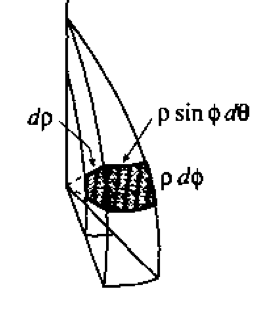
\includegraphics [scale=0.4] {sphere_dV.png} \end{center}

Notice that the top of the box is $\rho \sin \phi \ d\theta = r d\theta$, varying with $\phi$, while the sides do not depend on the polar angle but are just $\rho \ d\phi$.

We might as well check this
\[ V = \iiint dV = \int_{\theta = 0}^{2\pi} \ \int_{\phi=0}^{\pi} \ \int_{\rho=0}^{a} \rho^2 \sin \phi \ d \rho \ d \phi \ d \theta \]
\[=  \int_{\theta = 0}^{2\pi} \ \int_{\phi=0}^{\pi}  \frac{1}{3} a^3 \sin \phi \ d \phi \ d \theta \]
\[=  \int_{\theta = 0}^{2\pi} \ \frac{1}{3} a^3 (-\cos \phi) \bigg |_{0}^{\pi}   \ d \theta \]
\[=  \int_{\theta = 0}^{2\pi} \ \frac{1}{3} a^3 (2)   \ d \theta \]
\[=  \frac{1}{3} a^3 (2)(2 \pi) \]
\[=  \frac{4}{3} \pi a^3 \]
which seems to be correct.

\subsection*{surface}

How about parametrizing the surface of the sphere?  In this case $\rho$ is a constant, and we will have only two variables, similar to longitude and latitude.
The standard parametrization of the (unit) sphere is
\[ \mathbf{r}(\phi, \theta) = \ <\sin \phi \cos \theta, \sin \phi \sin \theta, \cos \phi> \]
\[ \mathbf{r}_{\phi} = \ < \cos \phi \cos \theta, \cos \phi \sin \theta, -\sin \phi > \ \]
\[ \mathbf{r}_{\theta} = \ < -\sin \phi \sin \theta, \sin \phi \cos \theta, 0 > \ \]
The cross-product is
\[ \mathbf{r}_{\phi} \times \mathbf{r}_{\theta} =  \]
\[ < -\sin^2 \phi \cos \theta, \sin^2 \phi \sin \theta, \sin \phi \cos \phi> \]
If we want 
\[ |\mathbf{r}_{\phi} \times \mathbf{r}_{\theta} | = \sqrt{\sin^4 \phi \cos^2 \theta + \sin^4 \phi \sin^2 \theta + \sin^2 \phi \cos^2 \phi} \]
\[ = \sqrt{\sin^4 \phi + \sin^2 \phi \cos^2 \phi} \]
\[ = \sqrt{\sin^2 \phi} \]
\[ = \sin \phi \]

In my writeup of the first part of Schey's book (chapter 2), we saw that the normal vector to a surface is

\[  \hat{\mathbf{n}} = \frac{\mathbf{u} \times \mathbf{v}}{| \mathbf{u} \times \mathbf{v} |} \]

Dividing the cross-product above by its absolute value we get
\[ \frac{\mathbf{r}_{\phi} \times \mathbf{r}_{\theta} }{ | \mathbf{r}_{\phi} \times \mathbf{r}_{\theta} | } \]
\[ = \frac{1}{\sin \phi} \ < -\sin^2 \phi \cos \theta, \sin^2 \phi \sin \theta, \sin \phi \cos \phi> \ \]
\[ =  \ < -\sin \phi \cos \theta, \sin \phi \sin \theta, \cos \phi> \ \]
\[ = \ <-x,-y,-z> \ \]

???



\end{document}  